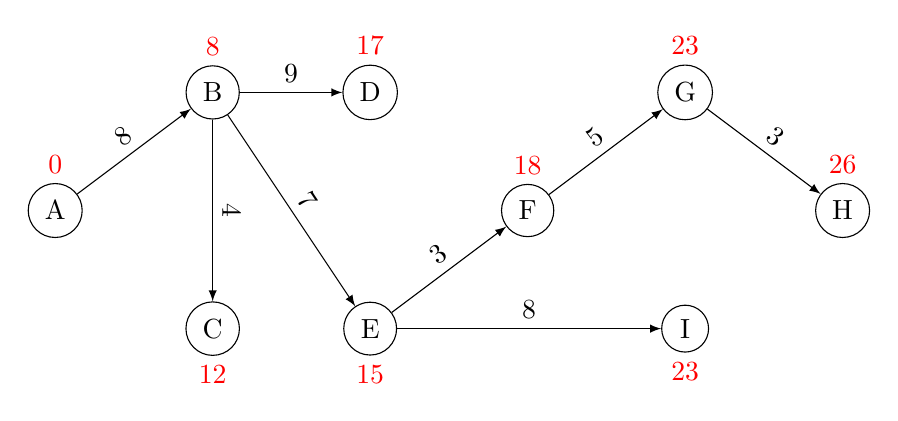
\begin{tikzpicture}
  \node[shape=circle, draw=black, label={[red]$0$}] (1) at (0, 0) {A};
  \node[shape=circle, draw=black, label={[red]$8$}] (2) at (2, 1.5) {B};
  \node[shape=circle, draw=black, label={[red]below:$12$}] (3) at (2, -1.5) {C};
  \node[shape=circle, draw=black, label={[red]$17$}] (4) at (4, 1.5) {D};
  \node[shape=circle, draw=black, label={[red]below:$15$}] (5) at (4, -1.5) {E};
  \node[shape=circle, draw=black, label={[red]$18$}] (6) at (6, 0) {F} ;
  \node[shape=circle, draw=black, label={[red]$23$}] (7) at (8, 1.5) {G};
  \node[shape=circle, draw=black, label={[red]$26$}] (8) at (10, 0) {H};
  \node[shape=circle, draw=black, label={[red]below:$23$}] (9) at (8, -1.5) {I} ;
  \draw[-latex] (1) -- (2) node[midway, sloped, above] {8};
  \draw[-latex] (2) -- (4) node[midway, sloped, above] {9};
  \draw[-latex] (2) -- (5) node[midway, sloped, above] {7};
  \draw[-latex] (2) -- (3) node[midway, sloped, above] {4};
  \draw[-latex] (5) -- (6) node[midway, sloped, above] {3};
  \draw[-latex] (5) -- (9) node[midway, sloped, above] {8};
  \draw[-latex] (6) -- (7) node[midway, sloped, above] {5};
  \draw[-latex] (7) -- (8) node[midway, sloped, above] {3};
\end{tikzpicture}
